%%=============================================================================
%% Technische Analyse
%%=============================================================================
\chapter{Technische Analyse}
\label{ch:technischeanalyse}

\section{Architectuur}
Voor het proof of concept zullen 3 applicaties worden gemaakt:
\begin{enumerate}
    \item D365FO applicatie met eigen model ('chtbt')
    \item C\# .NET webapplicatie voor authenticatie
    \item Implementatie in het MS Bot Framework
\end{enumerate}
\begin{figure}[h]
    \centering
    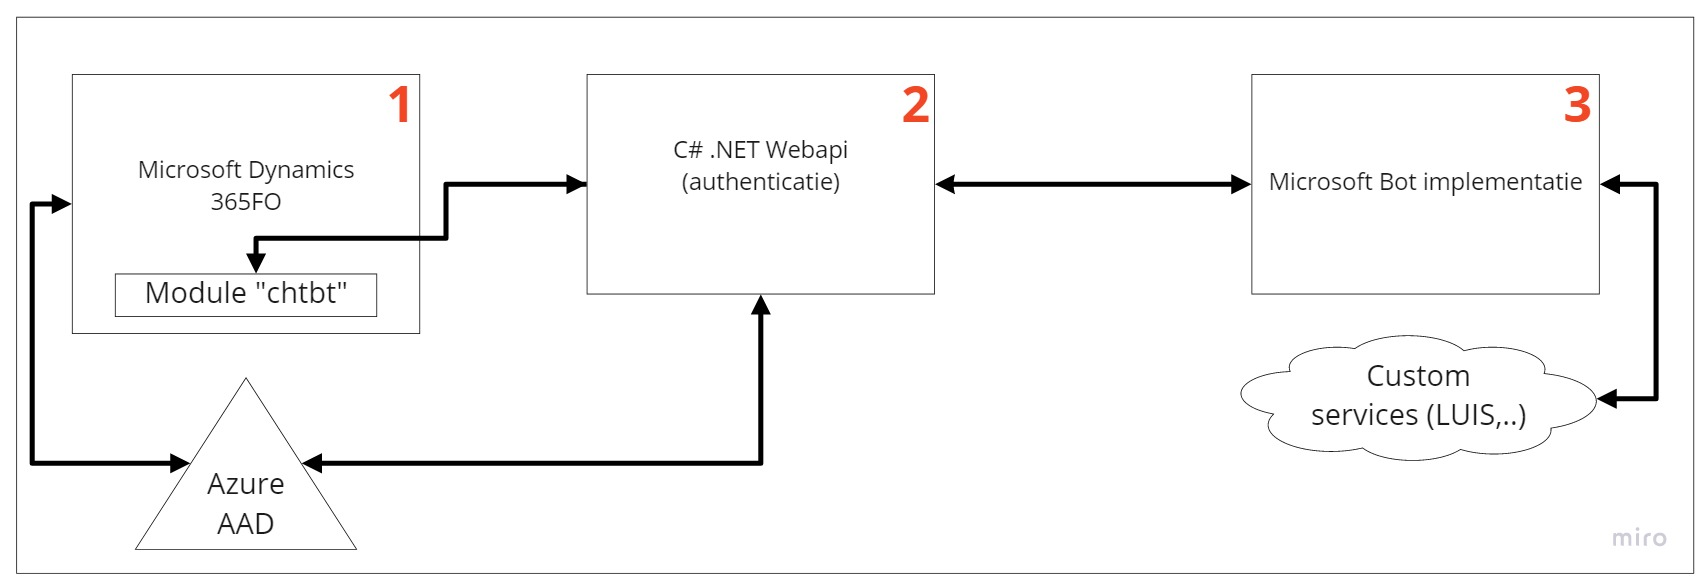
\includegraphics[width=1\textwidth]{img/ApplicatieArchitectuur}
    \caption{Applicatie architectuur}
\end{figure}
De eerste applicatie dient voor het programmeren van custom services binnen D365F0. Hiervoor zal een apart model gebouwd worden, genaamd 'chtbt' (afkorting voor chatbot). Binnen deze applicatie zal bestaande logica uit D365FO gebruikt, en beschikbaar gesteld worden d.m.v. een webservice. 

De tweede applicatie zal vervolgens connecteren met de eerste, en als communicatiemiddel dienen tussen de eerste en de derde applicatie. De reden dat hiervoor een aparte webapplicatie werd gebouwd is om de scheiding van taken en verantwoordelijkheden duidelijk af te bakenen per applicatie. Zo zal het authenticatiegedeelte (zie later) in deze omvat worden om gevoelige informatie (verbindingssleutels Azure, etc.) te verbergen voor de buitenwereld. 

Tenslotte zal uiteraard ook een chatbot gebouwd worden. Als deze dan wilt communiceren met D365FO om bepaalde CRUD-operaties uit te voeren, hoeft het enkel requests te versturen naar de authenticatie applicatie.

\section{Ontwikkel omgeving}
De ontwikkeling van het POC gebeurt volledig in de cloud, en dit op een Remote Desktop die draait op Lifecycle Services van Microsoft. Dit is een portaal waar meerdere mensen kunnen samenwerken, en dat de gebruiker assisteert in het beheren van de applicatie lifecycles van de verschillende D365FO implementaties.
Een schematische voorstelling:

\begin{figure}[H]
    \centering
    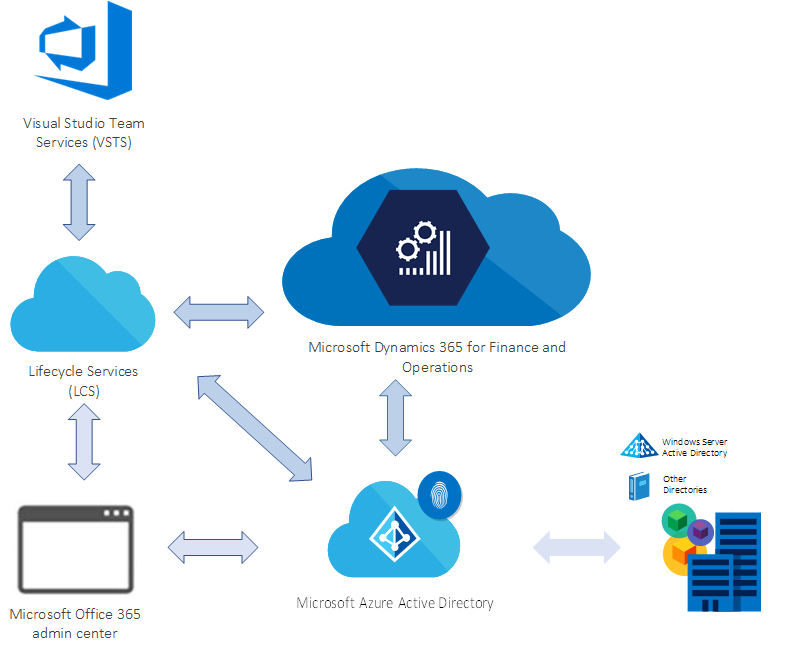
\includegraphics[width=0.8\textwidth]{img/lcsCloudArchitecture.png}
    \caption{Microsoft Lifecycle Services cloud architectuur}
\end{figure}

Aangezien dit proof of concept veel webrequests omvat, wordt er voor gekozen om deze eerst via de localhost te ontwikkelen. In een volgende stap zullen deze dan gehost worden. 

\section{Demo omgeving}
Wat betreft demo's van het poc zullen deze steeds 100\% in-cloud uitgevoerd worden. Dit wil zeggen dat alledrie de applicaties gehost zullen worden op hun respectievelijke webadressen, en de bot dus van eender waar bereikbaar, en bruikbaar is. 

De webadressen hiervoor zijn 
Insert finale webadressen
%%TODO 

\section{Authenticatie}
De authenticatie tussen Dynamics 365FO en de chatbot vereiste een aparte applicatie. Dit omdat de authenticatie volledig via Azure AAD verloopt. De authenticatie app werd geregistreerd binnen de D365FO Azure AAD applicaties (in D365FO: dashboard -> Azure Active Directory Applications). In D365FO ziet dit er als volgt uit: 
\begin{figure}[H]
    \centering
    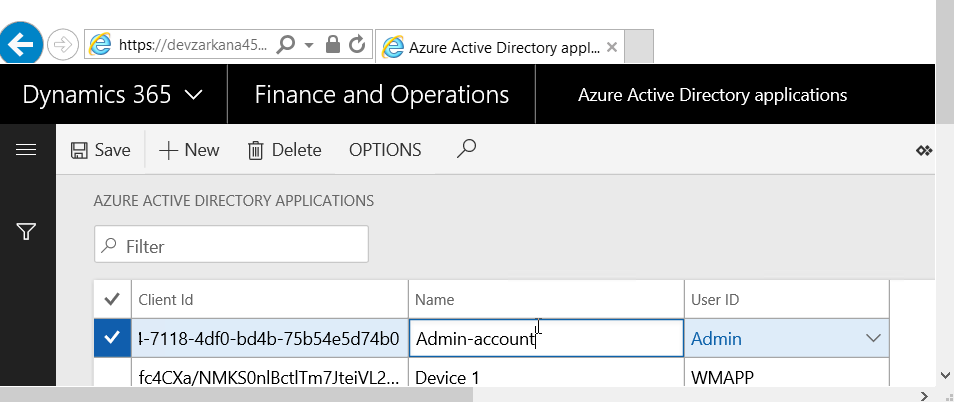
\includegraphics[width=1\textwidth]{img/impersination.png}
    \caption{Microsoft Lifecycle Services cloud architectuur}
\end{figure}
Nadat dit gebeurd is, kan er geconnecteerd worden met D365FO van buitenaf adhv. impersination. 
Dit wil zeggen dat wanneer iemand van buitenaf wilt inloggen op een d365FO omgeving, deze eerst moet inloggen op Azure om een Authorization Token te ontvangen. Vervolgens kan de gebruiker dan toegang aanvragen aan de resource (D365FO), om zo een Acces Token te kunnen bekomen. Als deze werd toegekend kan de Acces Token meegestuurd worden met alle volgende requests naar D365FO. Deze zal immers aan de Dynamics kant gevalideerd worden om dan toegang toe te kennen of te weigeren naargelang de situatie die zich voordoet. In onderstaande afbeelding wordt dit proces schematisch samengevat.

\begin{figure}[H]
    \centering
    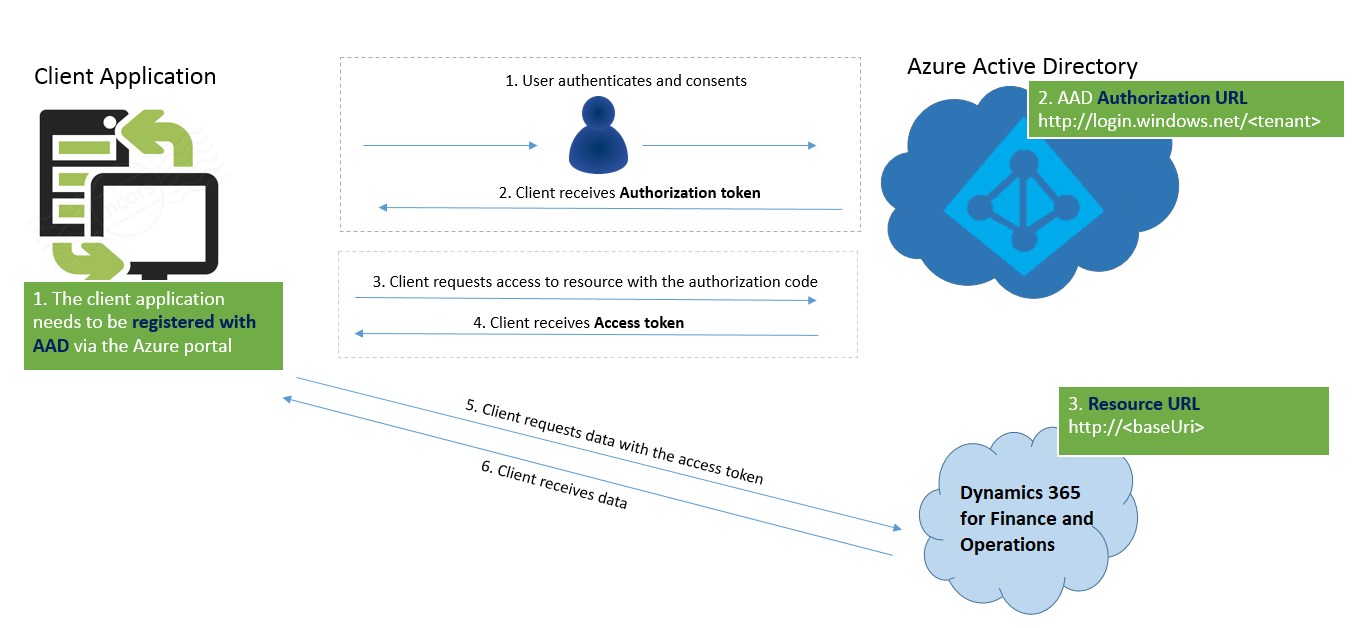
\includegraphics[width=1\textwidth]{img/aadAuthenticationArchitecture.png}
    \caption{D365FO authenticatie mbv Azure Active Directory}
\end{figure}
\subsection{Azure resources}
op het einde
\section{Data model}
Binnen D365FO zullen custom klassen en methodes gebruikt worden bovenop de reeds bestaande. De reden hiervoor is om op efficiënte manier informatie te kunnen versturen in webrequests. De bestaande klassen in D365FO zou een vorm van overkill zijn, omdat deze heel veel data bevatten die niet relevant is voor het poc. Deze klassen zullen vervolgens geserialiseerd verstuurd worden als JSON-objecten. 

\subsection{Json 2 Csharp}
De in D365FO (X++) geïmplementeerde klassen zullen vervolgens ook nodig zijn in de authenticatie app (C\#). Dit zodat de geserialiseerde JSON objecten gedeserialiseerd kunnen worden in C\# objecten. Hiervoor kan men er voor kiezen om alles dubbel te programmeren, wat dus ook dubbel werk betekent. Een andere optie is echter om de JSON strings te gebruiken voor de conversie. Hier zijn verschillende sites en tools voor, waarvan Json2Csharp.com een voorbeeld is. 
In onderstaande afbeelding wordt geïllustreerd hoe dit in zijn werk gaat. De geserialiseerde JSON string kan integraal geplakt worden, waarna de tool automatisch C\# klassen zal creëren die op hun beurt slechts gekopieerd en geplakt moeten worden in een nieuwe lege C\# klasse. 
\begin{figure}[H]
    \centering
    \includegraphics[width=1\textwidth]{img/json2Csharp.png}
    \caption{Json2Csharp voorbeeld}
\end{figure}

\section{UML}